\documentclass[dvipdfmx]{jsarticle}

\usepackage{ascmac}
\usepackage{url}
\usepackage[dvipdfmx]{hyperref}
\usepackage{pxjahyper}
\usepackage[dvipdfmx]{graphicx}
\usepackage{float}
\usepackage{listings,jlisting}

\hypersetup{
  colorlinks=true,
  urlcolor=cyan,
  linkcolor=black
}

\lstset{
  basicstyle={\ttfamily},
  identifierstyle={\small},
  commentstyle={\smallitshape},
  keywordstyle={\small\bfseries},
  ndkeywordstyle={\small},
  stringstyle={\small\ttfamily},
  frame={tb},
  breaklines=true,
  columns=[l]{fullflexible},
  numbers=left,
  xrightmargin=0zw,
  xleftmargin=3zw,
  numberstyle={\scriptsize},
  stepnumber=1,
  numbersep=1zw,
  lineskip=-0.5ex
}

\begin{document}

\section{実験目的・課題}

ファイル入出力、正規表現について学ぶ

\begin{itemize}
  \item テストを行った結果表を読み込み集計する
  \item 個人の名前と教科ごとの平均点を表示するプログラムを作成する
  \item 成績表はTab区切りファイルで保存されているとする
  \item 正規表現を使い入力エラーに対応する
  \item 教科数を増やした場合に対応する
  \item 成績クラスを継承した新しいクラスを作成する
  \item 継承したクラスにおいてメソッドのオーバーライドをする
\end{itemize}

以上の7つのことを行う。
入力の成績表は表1,2,3に示す。

\begin{table}[H]
  \begin{tabular}{cccccc}
    Number & Name & Score1 & Score2 & Score3 & Score4 \\ \hline
    1 & Michael & 75 & 86 & 89 & 31 \\
    2 & Emma & 74 & 63 & 70 & 48 \\
    3 & Hannah & 73 & 45 & 82 & 31 \\
    4 & Emily & 40 & 30 & 49 & 48 \\
    5 & Daniel & 46 & 59 & 47 & 70 \\
    6 & Oliver & 59 & 26 & 61 & 44 \\
    7 & Mia & 74 & 64 & 62 & 72 \\
    8 & James & 86 & 61 & 51 & 78 \\
    9 & Charlotte & 85 & 50 & 66 & 61 \\
    10 & Luna & 52 & 72 & 57 & 56 \\
    11 & Mason & 60 & 80 & 50 & 49 \\
  \end{tabular}
  \centering
  \caption{4教科成績表エラーなし}
  \label{in1}
\end{table}

\begin{table}[H]
  \begin{tabular}{cccccc}
    Number & Name & Score1 & Score2 & Score3 & Score4 \\ \hline
    1 & Michael & 75 & 86 & 89 & 31 \\
    2 & Emma & 74 & 63 & 70 & �S8 \\
    3 & Hannah & 73 & 45 & 82 & 31 \\
    4 & Emily & 40 & 30 & 40 \\
    5 & Daniel & 46 & 59 & 47 & 70 \\
    6 & Oliver & 59 & 2.6 & 61 & 44 \\
    7 & Mia & 74 & 64 & 62 \\
    8 & James & 86 & 61 & 51 & 78 \\
    9 & Charlotte & 85 & 50 & 66 & 611 \\
    10 & Luna & 52 & 72 & �T7 & 56 \\
    11 & Mason & 60 & 80 & 50 & 49 \\
  \end{tabular}
  \centering
  \caption{4教科成績表エラーあり}
  \label{in2}
\end{table}

\begin{table}[H]
  \begin{tabular}{cccccccc}
    Number & Name & Score1 & Score2 & Score3 & Score4 & Score5 \\ \hline
    1 & Michael & 75 & 86 & 89 & 31 & 39 \\
    2 & Emma & 74 & 63 & 70 & �S8 & 88 \\
    3 & Hannah & 73 & 45 & 82 & 31 & 26 & 26 \\
    4 & Emily & 40 & 30 & 48 & 40 \\
    5 & Daniel & 46 & 59 & 47 & 70 & 72 \\
    6 & Oliver & 59 & 26 & 61 & 44 & 65 \\
    7 & Mia & 74 & 64 & 62 \\
    8 & James & 86 & 61 & 51 & 78 & 60 \\
    9 & Charlotte & 85 & 50 & 66 & 611 & 79 \\
    10 & Luna & 52 & 72 & �T7 & 56 & 85 \\
    11 & Mason & 60 & 80 & 50 & 49 & 58 \\
  \end{tabular}
  \centering
  \caption{5教科成績表エラーあり}
  \label{in3}
\end{table}

\section{基礎知識}
\subsection{ファイル入力}
\subsubsection{Javaの標準入出力}
キーボードからなどの標準入力は、InputStreamというバイト列を保持する型で受け取る。
普通、このインスタンスを独自生成することはなく、
Javaの標準APIであるSystemクラスのメンバ変数inを使用する。
このとき直接文字列で受け取るのではなくバイト列で受け取るのは文字エンコードによる制約を受けないためである。

このバイトストリームを文字ストリームへ変換するのがInputStreamReaderである。
バイトを読み込み指定されたcharsetを使い文字にデコードすることが出来る。
charsetとは、16ビットUnicodeコード単位のシーケンスとバイト・シーケンス間のマッピングをすることが出来るものである。
InputStreamReaderのread()メソッド(int read(void))を呼び出すたびにバイト入力ストリームから
1バイト読み込まれ文字へ変換される。以下のプログラムは、標準入力を1文字読み込み出力するものである。

\begin{lstlisting}[caption=1文字読み込み]
  import java.io.*;

  public class main{
    public static void main(String args[]){
      InputStream is = System.in;
      InputStreamReader reader = new InputStreamReader(is);
      try{
        int n = reader.read();
        System.out.println(n);
      }catch(IOException err){
        System.out.println(err);
      }
    }
  }
\end{lstlisting}

このプログラムの入力に全角の'あ'や半角の"ab"を与えると、それぞれ"12354"や"97"が
出力された。また、9行目をSystem.out.println((char)n);のようにか書き換え
同じ入力を与えたところ、'あ','a'が出力された。つまり、read()メソッドは入力を
1文字読み取りそれの文字コードを返していることがわかる。

この文字型入力ストリームをバッファリングすることによって
テキストを効率よく読み込むことをできるようにするものがBufferedReaderクラスである。
以下のプログラムは1行読み込み、それを出力することが出来る。

\begin{lstlisting}[caption=1行読み込み]
  BufferedReader reader = new BufferedReader(new InputStreamReader(System.in));
  try{
    String line = reader.readLine();
    System.out.println(line);
  }catch(IOException err){
    System.out.println(err);
  }
\end{lstlisting}

出力では、OutputStreamクラスの出力ストリームがバイトストリームを受け付け、特定の相手に送る。
PrintStreamクラスはそのプラットフォームのデフォルト文字セットを使用してバイトに変換し、
出力ストリームへ出力するクラスである。System.out.println()のprintln()メソッドは
このクラスが提供している。バイトではなく文字を書き込むことが必要な状況ではPrintWriterを使用する。
例えば、以下のように使用する。

\begin{lstlisting}[caption=1行出力]
  public static void main(String args[]){
    OutputStream os = System.out;
    PrintStream writer = new PrintStream(os);
    writer.println("sample output");
  }
\end{lstlisting}

\subsubsection{ファイルからの入力}

Javaでは、java.io.Fileクラスによってファイルやディレクトリを1つのオブジェクトとして扱うことができる。
ファイル入力でも標準入力の時と同じようにFileInputStream,FileReaderによってファイルから入力バイトを取得することが出来る。
oracleのjava docによるとrawバイトのストリームを読み込むときにFileInputStreamが、
文字ストリームを読み込むときにはFileReaderが推奨されている。

標準入出力でBufferedReader(InputStreamReader(InputStream))のようにしたように
ファイル入力ではBufferedReader(FileReader(File))とすることで
標準入力と同様に書くことが出来る。以下に例を示す。

\begin{lstlisting}[caption=ファイル入力]
  try{
    File file = new File("sample.txt");
    FileReader fr = new FileReader(file);
    BufferedReader br = new BufferedReader(fr);
    System.out.println(br.readLine());
  }catch(FileNotFoundException err){
    System.out.println(err);
  }catch(IOException err){
    System.out.println(err);
  }
}
\end{lstlisting}

BufferedReader(InputStreamReader(FileInputStream(File)))としても同様である。

\subsection{例外処理}

ゼロ除算や配列外参照などを行うとJavaでは例外として処理を中断させる。
例外処理とは、プログラム上でそのような事態が発生したときにどう対処するかを記述するものである。

Javaの例外は、Throwableクラスを継承したオブジェクトをスローすることで発生する。
例外としてありうるものは
\begin{itemize}
  \item Exception
  \begin{itemize}
    \item ex. IOException,ClassNotFound
  \end{itemize}
  \item RuntimeException
  \begin{itemize}
    \item ex. IndexOutOfIndex
  \end{itemize}
  \item Error
  \item \begin{itemize}
    \item ex. VirtualMachineError
  \end{itemize}
\end{itemize}
の3つである。

実際にスローされる例外クラスは全てがThrowableクラスを直接継承しているのではなく、
図\ref{throwable}のようにRuntimeExceptionはExceptionを継承するようになっている。
\begin{figure}[H]
  \centering
  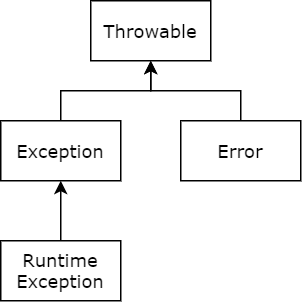
\includegraphics[width=0.3\hsize]{../pic/1.png}
  \caption{例外クラスの継承}
  \label{throwable}
\end{figure}

Exceptionがスローされるコードはコンパイル時に例外処理の実装が強制され、
RuntimeExceptionは強制されない。
Errorは処理の継続が難しい致命的な場合であるため、例外処理を記述することはできない。

例外処理の構文は以下のようになる。
\begin{lstlisting}[caption=例外処理の構文]
  try{
    例外が起こりうる処理
  }catch(例外の型 変数名){
    例外が起きた時の処理
  }finary{
    最後に実行される処理
  }
\end{lstlisting}
起こりうる例外が一つとは限らないのでcatchは複数書くこともできる。また、finaryは書いても書かなくてもよい。
また、スローされた例外をキャッチせずにそのままスローすることもでき、ソースコード4はソースコード6のように書ける。
\begin{lstlisting}[caption=例外処理を行わずにスローする]
  import java.io.*;

  public class main{
    public static void main(String args[]) throws IOException{
      try{
        File file = new File("sample.txt");
        FileReader fr = new FileReader(file);
        BufferedReader br = new BufferedReader(fr);
        System.out.println(br.readLine());
      }catch(FileNotFoundException err){
        System.out.println(err);
      }
    }
  }
\end{lstlisting}

\subsection{正規表現}

正規表現は文字列として指定し、Patternクラスのインスタンスにコンパイルする必要がある。
その結果のパターンを使用して任意の文字シーケンスを正規表現とマッチできる
Matcherオブジェクトを生成できる。通常、以下のように使用する。
\begin{lstlisting}[caption=正規標準の呼び出し方,label=regex1]
  Pattern p = Pattern.compile("a*b");
  Matcher m = p.matcher("aaaab");
  boolean b = m.matches();
\end{lstlisting}
また次の文はソースコード\ref{regex1}と等価である。
\begin{lstlisting}
  boolean b = Pattern.matches("a*b","aaaab");
\end{lstlisting}
ただし、マッチを繰り返す場合、コンパイル済みパターンを再利用したほうが効率が良い。

以下に正規表現で使うことのできる構文を示す。
\begin{table}[H]
  \begin{tabular}{cc}
    文字x & x \\
    任意の文字 & . \\
    バックスラッシュ文字 & \textbackslash\textbackslash  \\
    タブ文字 & \textbackslash t \\
    改行文字 & \textbackslash n \\
    a,bまたはc & [abc] \\
    a,b,c以外の文字 & [\textasciicircum abc] \\
    a-zの文字 & [a-z] \\
    a-zあるいはA-Z & [a-zA-Z] \\
    b,cを除くa-z & [a-z\&\&[\textasciicircum bc]] \\
    小文字の英字(a-z) & \textbackslash p\{Lower\} \\
    大文字の英字(A-Z) & \textbackslash p\{Upper\} \\
    英字(a-zA-Z) & \textbackslash p\{Alpha\} \\
    空白またはタブ & \textbackslash p\{Blank\} \\
  \end{tabular}
  \centering
  \caption{正規表現の文字クラス}
\end{table}
\begin{table}[H]
  \begin{tabular}{cc}
    \emph{最長一致} \\
    X、1または0回 & X? \\
    X、0回以上 & X* \\
    X、1回以上 & X+ \\
    X、n回 & X\{n\} \\
    X、n回以上 & X\{n,\} \\
    X、n回以上、m回以下 & X\{n,m\} \\
    \emph{最短一致} \\
    X、1または0回 & X?? \\
    X、0回以上 & X*? \\
    X、1回以上 & X+? \\
    X、n回 & X\{n\}? \\
    X、n回以上 & X\{n,\}? \\
    X、n回以上、m回以下 & X\{n,m\}? \\
    \emph{論理演算子} \\
    Xの直後にY & XY \\
    XまたはY & X \textbar Y \\
    X、前方参照を行う正規表現グループ & (X) \\
  \end{tabular}
  \centering
  \caption{最長(最短)一致数量子、論理演算子}
\end{table}


最長一致と最短一致とは、文字列"abbbc"に対して"ab+"のマッチを考えた時、
最長一致では"abbb"がマッチするのに対し、最短一致("ab+?")では"ab"がマッチする。

前方参照を行う正規表現グループは()によって番号を付けることができる。例えば
((A)(B(C)))は次の4つのグループに分けられる。
\begin{enumerate}
  \setcounter{enumi}{-1}
  \item ((A)(B(C)))
  \item (A)
  \item (B(C))
  \item (C)
\end{enumerate}

グループ0は常に全体を指す。
前方参照を行う正規表現グループが分類されたあと、入力シーケンスの各部分シーケンスが
これらのグループをマッチされ、マッチするたびに部分シーケンスが保存される。
正規表現グループの部分シーケンスは、前方参照として表現内であとで使用することが出来る。
また、マッチ終了後に各部分を取り出すことが出来る。


\section{実装方法}
\subsection{入力文字列の解析}

まず、2.1.2ソースコード4に基づいて入力ファイルを読み込む。
入力ファイルのパスはコンストラクタで与えるものとした。
ただし入力の一番上の行はカラム名であるため、最初の1行は読み飛ばす処理を入れる。
また、複数行の入力があるため入力がなくなるまでwhile文で読み続ける。
全ての入力を受け取った後にreadLine()を行うと返り値はnullであるため、
nullでない間処理を繰り返し続ける。
このとき発生しうる例外は、文字エンコードがサポートされていない、ファイルが存在しない、
入力に失敗する、の3つであるため、それぞれcatchしエラーメッセージを表示するようにする。
\begin{lstlisting}[caption=複数行の入力,label=impl1]
  File file = new File(this.path);
  BufferedReader br = new BufferedReader(new InputStreamReader(new FileInputStream(file), "UTF-8"));
  br.readLine();
  String line;
  while ((line = br.readLine()) != null) {
    seiseki tmp = this.parseSeiseki(line);
    if(tmp!=null)this.data.add(tmp);
  }
\end{lstlisting}

次に、読み込んだ1行が成績クラスの条件を満たしているか、入力が不正なデータではないか正規表現でチェックする。
入力行は、Number,Name,Score1,2,3,4の6つがTab区切りで与えられるはずである。
5教科の場合はScore5が追加され7つがTab区切りで与えられる。
これを正規表現で表すと以下のようになる。

\begin{lstlisting}[caption=入力行の構文解析に使用する正規表現,label=regex2]
  "([0-9]+) \\t ([A-Za-z]+) \\t ([0-9]+) \\t ([0-9]+) \\t ([0-9]+) \\t ([0-9]+)"
  "([0-9]+) \\t ([A-Za-z]+) \\t ([0-9]+) \\t ([0-9]+) \\t ([0-9]+) \\t ([0-9]+) \\t ([0-9]+)"
\end{lstlisting}

この正規表現のパターンの切り替えは、コンストラクタで何教科あるかを与えられるようにした。
このパターンにマッチしなければ入力行は正しくなく、nullを返す。
マッチした場合、正規表現グループの1にNumber、2にName、3から6あるいは7までにScoreが
格納されている。これをそれぞれMatcherクラスのString group(int)メソッドで取り出し
成績クラスのコンストラクタに渡し、それを返す。
この操作を行っているのがparseSeisekiである。

このように入力にエラーがないとして取り出されたものをArrayListにaddしていくことで
最終的に全てのデータを読み込むことが出来る。

全体の流れを図\ref{flowchart1}に示す。
\begin{figure}[H]
  \centering
  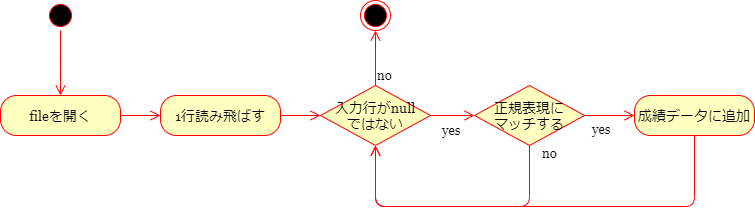
\includegraphics[width=0.9\hsize]{../pic/flow1.png}
  \caption{データ読み込みの流れ}
  \label{flowchart1}
\end{figure}

\subsection{教科ごとの平均点の算出}

教科数をN、正しい成績が入力された人数をM、j人目のi科目目を$A_{j,i}$をとして、
i教科目の平均点は
$\displaystyle n_i = \frac{1}{M}\sum_{j=0}^{M-1}A_{j,i}$
で計算することが出来る。

\subsection{成績クラスの継承}

成績クラスを継承した5教科用成績クラスをソースコード\ref{inheritance}に示す。
\begin{lstlisting}[caption=成績クラスを継承したクラス,label=inheritance]
  public class seiseki5 extends seiseki{
    public seiseki5(int num,String name,List<Integer> score){
      super(num,name,score);
    }
    @Override
    public double get_average(){
      double average = 0;
      for(int i=0;i<5;++i)average+=this.Scores.get(i);
      return average/5.0;
    }
}
\end{lstlisting}

コンストラクタはsuper()として継承の元となったスーパークラスのコンストラクタを呼び出すことができる。
個人の平均点を求めるメソッドを4教科のものから5教科のものにオーバーライドしている。
メソッドは「メソッド名+引数リスト」(この組み合わせをシグニチャという)で一意に特定し、
オーバーロードはシグニチャが同じになり、メソッド名が同じでもシグニチャが異なるものはオーバーロードという。


\section{結果と考察}
\subsection{4教科エラーなし}
4教科エラーなし入力を読み込んだ時の出力結果を図\ref{res1}に示す。
\begin{figure}[H]
  \centering
  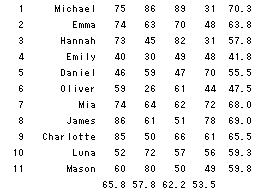
\includegraphics[width=0.6\hsize]{../pic/res1.png}
  \caption{4教科エラーなし入力の結果}
  \label{res1}
\end{figure}

表\ref{in1}と比べるとデータが正しく読み取れていることがわかる。
また、MichaelとScore1について平均点をPythonで計算したものを以下に示す。
この結果と比べると平均点が正しく計算出来ていることがわかる。
\begin{lstlisting}
  >>> def average(list):return sum(list)/len(list)
  ...
  >>> Michael=[75,86,89,31]
  >>> Score1=[75,74,73,40,46,59,74,86,85,52,60]
  >>> average(Michael)
  70.25
  >>> average(Score1)
  65.81818181818181
\end{lstlisting}

Michaelの平均点を図\ref{res1}と比べると
小数点以下2桁目を四捨五入して表示していると考えられる。
これは、少数の出力にJavaのStringのformatメソッドを使い、
String.format("\%5.1f",average);としているためである。
\%fは少数の出力を表し、5は5文字になるように先頭を空白で埋め、
.1は小数点以下1桁目まで出力するということである。

\subsection{4教科エラーあり}
図\ref{res2}に4教科エラーあり入力に対する出力を示す。
\begin{figure}[H]
  \centering
  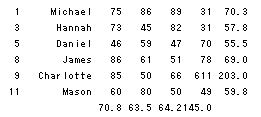
\includegraphics[width=0.6\hsize]{../pic/res2.png}
  \caption{4教科エラーあり入力の結果}
  \label{res2}
\end{figure}

これも計算して確かめると正しい答えが出力されていることがわかる。
CharlotteのScore4が611点と他と比べて非常に大きい数になっているため
Score3とScore4の平均点の間に空白が挟まらずに見にくくなってしまっている。
これを解決するためにはformatで幅が5文字ではなく6文字になるようにすればよい。

このテストの最大得点がわからないため611点はエラーではないと判断したがもし
テストの点数が100点より大きいものをエラーとするなら、"[0-9]+"という
パターンで得点を表現するのではなく、"[0-9]\{1,2\}\textbar100"とすることで、
0から9までの数が1桁または2桁、あるいは100のときのみに正規表現にマッチするため、
期待する動作ができると考えられる。
以上の2つの修正をした結果を図\ref{res2_2}に示す。
\begin{figure}[H]
  \centering
  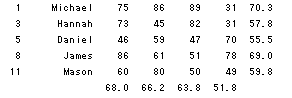
\includegraphics[width=0.7\hsize]{../pic/res2_2.png}
  \caption{4教科エラーあり入力の結果2}
  \label{res2_2}
\end{figure}

\subsection{5教科エラーあり}
5教科エラーあり入力、成績クラスを継承したものを使用したプログラムの実行結果を図\ref{res3}に示す。
このときプログラム中のseisekiという文字列を全てseiseki5というふうに置き換えなければならない。
しかし、これを眼で見て一つ一つ行うのはミスをする可能性が大きく、プログラムが大きければ
時間がかかってしまう。ここでNetBeansの置換という機能を使えば1つのファイルの中の
特定の文字列を一斉に別の文字列に置き換えることが出来るため、これを使用した。
\begin{figure}[H]
  \centering
  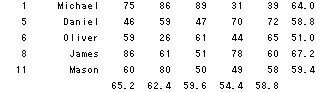
\includegraphics[width=0.7\hsize]{../pic/res3.png}
  \caption{5教科エラーあり入力の結果}
  \label{res3}
\end{figure}

4教科から5教科への切り替えのためにソースコード\ref{regex2}のように2つのパターンを
切り替えなければならない。入力が4教科か5教科しかないならばこれでもいいが
6,7,...と増えて言った場合パターンを書き直すあるいはコメントアウトなどするのは面倒である。
ここで、2つの正規表現に注目してみると、
"\textbackslash\textbackslash t ([0-9]\{1,2\}\textbar100)"
が繰り返される回数しか違いがないことがわかる。
よって、教科数をNとして、ソースコード\ref{regex3}のようにすることで
Nの数字を変えるだけで教科数の変更に対応できるようになる。
\begin{lstlisting}[caption=N教科の正規表現,label=regex3]
  String regex = "([0-9]+) \\t ([a-zA-Z]+)";
  for(int i=0;i<N;++i)
    regex += "\\t ([0-9]{1,2}|100)";
  Pattern ptn = Pattern.compile(regex);
\end{lstlisting}


\begin{thebibliography}{10} 
  \bibitem{1} Java SE API \& ドキュメント \\
  \url{https://www.oracle.com/jp/java/technologies/javase/documentation/api-jsp.html}
  \bibitem{2} IT専科 Java入門 \\
  \url{http://www.itsenka.com/contents/development/java/}
\end{thebibliography}


\end{document}